
\section{Charge extortion}
\label{chap5:sect:chargeExtortion}

\subsection{Logic considerations}
\label{chap5:sect:chargeExtortion:subsect:logicConsiderations}

\begin{figure}[htbp!]
    \centering
    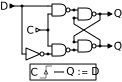
\includegraphics[width=0.6\textwidth]{5_faultModel/figures/dffLogic.pdf}
    \caption{D Flip-Flop logic schematic}
    \label{chap:5;fig:dffLogic}
\end{figure}
In order to understand electrically why faults occur, it is important to begin with logic considerations.
Nowadays, the vast majority of commercial ICs are sequential.
The main building block of a sequential IC is the Edge-Triggered D Flip-Flop (DFF).
Fig. \ref{chap:5;fig:dffLogic} presents the logic schematic of a DFF.
Because DFFs work on clock edges, it is interesting to target them at specific times when performing fault injection.
\textcolor{magenta}{Paragraphe à terminer, compléTer, revoir...}
%The block has two inputs and two outputs.
%This building block is ruled by a clock, input at C.
%At each rising edge of the clock, the output samples the input value.
%It is thus a memory cell, which stores at Q for a short amount of time the value present at D.
%What is important to remember here is that outside of the rising edge, any change at D is not seen at Q.
%Therefore, when performing fault injections, it is interesting to affect the value at D long enough to let the DFF sample an incorrect value.
This fault model has been proposed in \cite{emfiFF} for EMFI.

\textcolor{magenta}{Parler du fait que les circuits séquentiels échantillonnent périodiquement les valeurs des DFFs (registres). Du coup, si on change un niveau logique suffisamment longtemps pour qu'il perdure pendant l'échantillonnage, c'est gagné ! Faute !, sinon Non.}

\subsection{Charge extortion}
\label{chap5:sect:chargeExtortion:subsect:chargeExtortion}

\begin{figure}[H]
    \centering
    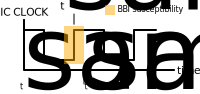
\includegraphics[width=15cm]{5_faultModel/figures/bbiFaultSusceptibility.pdf}
    \caption{BBI sampling fault susceptibility}
    \label{chap:5;fig:bbiSusc}
\end{figure}
With the previous fault model in mind, let's have deeper look at it.
Fig. \ref{chap:5;fig:bbiSusc} presents the sampling fault model we are going to discuss.
It states that to maximize fault creation, faults have to be injected during a specific period of time.
It is precisely located before and after every clock rising edge.